\documentclass[a4paper,twoside]{article}
\usepackage{blindtext}  
\usepackage{geometry}

% Chinese support
\usepackage[UTF8, scheme = plain]{ctex}

% Page margin layout
\geometry{left=2.3cm,right=2cm,top=2.5cm,bottom=2.0cm}


\usepackage{listings}
\usepackage{xcolor}
\usepackage{geometry}
\usepackage{amsmath}
\usepackage{float}
\usepackage{hyperref}

\usepackage{graphics}
\usepackage{graphicx}
\usepackage{subcaption}
\usepackage{epsfig}
\usepackage{float}

\usepackage{algorithm}
\usepackage[noend]{algpseudocode}

\usepackage{booktabs}
\usepackage{threeparttable}
\usepackage{longtable}
\usepackage{tikz}
\usepackage{multicol}
\usepackage{pgfplots}
\pgfplotsset{compat=1.9}
\pgfplotsset{
    myplotstyle/.style={
    legend style={draw=none, font=\small},
    legend cell align=left,
    legend pos=north east,
    ylabel style={align=center, font=\bfseries\boldmath},
    xlabel style={align=center, font=\bfseries\boldmath},
    x tick label style={font=\bfseries\boldmath},
    y tick label style={font=\bfseries\boldmath},
    scaled ticks=false,
    every axis plot/.append style={thick},
    },
}

% cite package, to clean up citations in the main text. Do not remove.
\usepackage{cite}

\usepackage{color,xcolor}

%% The amssymb package provides various useful mathematical symbols
\usepackage{amssymb}
%% The amsthm package provides extended theorem environments
\usepackage{amsthm}
\usepackage{amsfonts}
\usepackage{enumerate}
\usepackage{enumitem}
\usepackage{listings}
\usepackage{minted}


\usepackage{indentfirst}
\setlength{\parindent}{2em} % Make two letter space in the first paragraph
\usepackage{setspace}
\linespread{1.5} % Line spacing setting
\usepackage{siunitx}
\setlength{\parskip}{0.5em} % Paragraph spacing setting

% \usepackage[contents =22920202204622, scale = 10, color = black, angle = 50, opacity = .10]{background}

\renewcommand{\figurename}{图}
\renewcommand{\listingscaption}{代码}
\renewcommand{\tablename}{表格}
\renewcommand{\contentsname}{目录}
\floatname{algorithm}{算法}

\graphicspath{ {images/} }

%%%%%%%%%%%%%
\newcommand{\StudentNumber}{22920202204622}  % Fill your student number here
\newcommand{\StudentName}{熊恪峥}  % Replace your name here
\newcommand{\PaperTitle}{实验(一)体验Nachos下的并发程序设计}  % Change your paper title here
\newcommand{\PaperType}{学科实践} % Replace the type of your report here
\newcommand{\Date}{2023年3月28日}
\newcommand{\College}{信息学院}
\newcommand{\CourseName}{操作系统}
%%%%%%%%%%%%%

%% Page header and footer setting
\usepackage{fancyhdr}
\usepackage{lastpage}
\pagestyle{fancy}
\fancyhf{}
% This requires the document to be twoside
\fancyhead[LO]{\texttt{\StudentName }}
\fancyhead[LE]{\texttt{\StudentNumber}}
\fancyhead[C]{\texttt{\PaperTitle }}
\fancyhead[R]{\texttt{第{\thepage}页,共\pageref*{LastPage}页}}


\title{\PaperTitle}
\author{\StudentName}
\date{\Date}

\algnewcommand\algorithmicinput{\textbf{Input:}}
\algnewcommand\algorithmicoutput{\textbf{Output:}}
\algnewcommand\Input{\item[\algorithmicinput]}%
\algnewcommand\Output{\item[\algorithmicoutput]}%

\usetikzlibrary{positioning, shapes.geometric,arrows,automata}


\begin{document}
	
%%%%%%%%%%%%%%%%%%%%%%%%%%%%%%%%%%%%%%%%%%%%
\makeatletter % change default title style
\renewcommand*\maketitle{%
	\begin{center} 
		\bfseries  % title 
		{\LARGE \@title \par}  % LARGE typesetting
		\vskip 1em  %  margin 1em
		{\global\let\author\@empty}  % no author information
		{\global\let\date\@empty}  % no date
		\thispagestyle{empty}   %  empty page style
	\end{center}%
	\setcounter{footnote}{0}%
}
\makeatother
%%%%%%%%%%%%%%%%%%%%%%%%%%%%%%%%%%%%%%%%%%%%
	
	
\thispagestyle{empty}

\vspace*{1cm}

\begin{figure}[htb]
	\centering
	
\includegraphics[width=4.0cm]{logo.png}
\end{figure}

\vspace*{1cm}

\begin{center}
	\Huge{\textbf{\PaperType}}
	
	\Large{\PaperTitle}
\end{center}

\vspace*{1cm}

\begin{table}[H]
	\centering	
	\begin{Large}
		\renewcommand{\arraystretch}{1.5}
		\begin{tabular}{p{3cm} p{5cm}<{\centering}}
			姓\qquad 名 & \StudentName  \\
			\hline
			学\qquad号 & \StudentNumber \\
			\hline
			日\qquad期 & \Date  \\
			\hline
			学\qquad院 & \College  \\
			\hline
			课程名称 & \CourseName  \\
			\hline
		\end{tabular}
	\end{Large}
\end{table}

\newpage

\title{
	\Large{\textcolor{black}{\PaperTitle}}
}

\maketitle
	
\tableofcontents
 
\newpage
\setcounter{page}{1}

\begin{spacing}{1.2}

\section{使用Docker安装Nachos}

\subsection{构建容器}

由于Nachos需要使用较旧的工具链,因此在现代操作系统上使用Nachos可能会遇到一些问题。
然而专为Nachos安装旧版本的虚拟机比较麻烦,因此为了方便开发、方便阅读和修改代码,可以使用Docker安装Nachos。

首先,由于Docker Hub没有现成的容器,要先编写Dockerfile,然后使用Docker build命令构建容器。如代码~\ref{code:dockerfile}
\begin{listing}[htb]
	\caption{Dockerfile}
	\label{code:dockerfile}
    \begin{minted}{dockerfile}
ARG UPSTREAM_IMAGE=i386/ubuntu:bionic

FROM ${UPSTREAM_IMAGE}

# install compiler
RUN apt update && \
    apt install -y ed csh gdb build-essential && \
    apt clean -y && \
    rm -rf /var/lib/apt/lists/*

# change workspace
WORKDIR /workspace

ENTRYPOINT [ "/bin/bash" ]
	\end{minted}
\end{listing}
然后使用命令
\begin{quotation}
	\texttt{docker buildx build -t nachos  .}
\end{quotation}
就可以按照Dockerfile进行构建。

\subsection{创建实例}

接下来,可以使用Docker创建一个容器的实例来运行Nachos。
运行命令
\begin{quotation}
	\texttt{docker run -v \$(pwd):/workspace -it nachos}
\end{quotation}
就可以使用刚才构建的容器创建一个容器的实例,并将容器的/workspace目录映射到当前目录。
在Docker Desktop中可以看到刚才创建的容器实例。如图~\ref{fig:docker}所示。
\begin{figure}[htb]
	\centering
	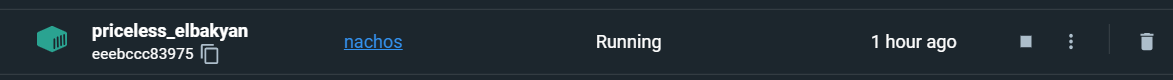
\includegraphics[width=0.8\textwidth]{images/docker.png}
	\caption{Docker Desktop}
	\label{fig:docker}
\end{figure}
容器在Running状态,说明容器已经启动。在Docker Desktop中可以打开终端、进行配置等操作,
但是为了更好地开发,可以使用VSCode连接容器进行开发。

\subsection{配置VSCode}

VSCode有完善的远程开发功能,可以连接到容器进行开发。在Remote Explorer中选择Containers,
刷新,就可以看见刚刚创建的容器实例,如图~\ref{code:vscodecont}
然后右键点击“Attach to Container”,选择刚才创建的容器实例,就可以连接到容器进行开发了。
\begin{figure}[htb]
	\centering
	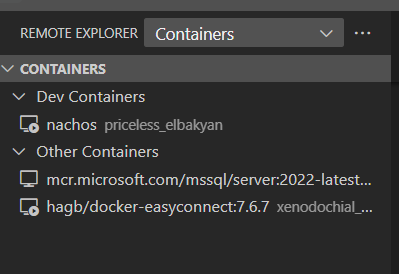
\includegraphics[width=0.4\textwidth]{images/vscodecnt.png}
	\caption{VSCode Containers}
	\label{code:vscodecont}
\end{figure}

在VSCode终端中可以编译代码,如图~\ref{fig:build}。绝大多数模块都能成功编译,可以支持进行正常的实验,
由于编译器版本还是较高,\texttt{tests}目录下有少数几个模块无法编译,但是不影响实验。可以在Makefile中
移除它们,或者忽略相关的报错。
\begin{figure}[htb]
	\centering
	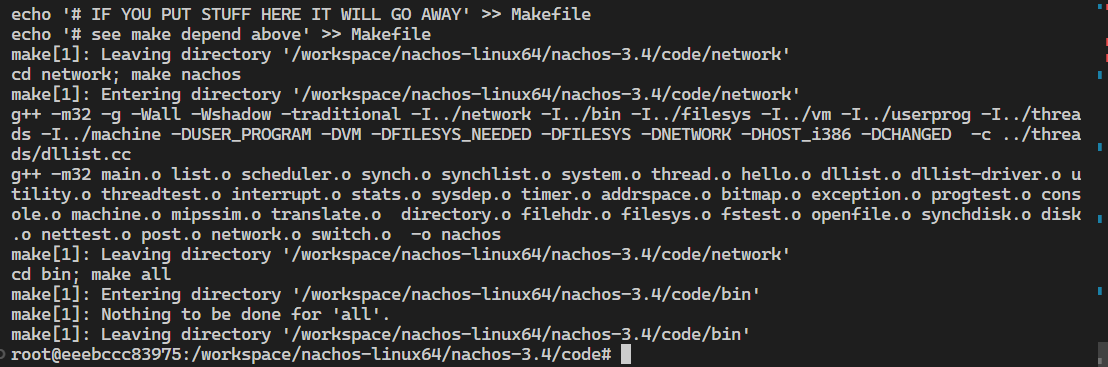
\includegraphics[width=0.8\textwidth]{images/build.png}
	\caption{Build Nachos}
	\label{fig:build}
\end{figure}

在\texttt{Makefile.common}中的THREAD\_C,THREAD\_H,和THREAD\_O中分别加入
hello.c, hello.h和hello.o,然后在其中实现输出Hello的函数,如代码~\ref{code:hello},
然后在\texttt{ThreadTest}中调用,可见在Nachos中添加的模块也可以正常运行。如图~\ref{fig:hello}。
\begin{listing}[htb]
	\caption{hello.c}
	\label{code:hello}
	\begin{minted}{c}
#include "copyright.h"
#include "system.h"

void hello()
{
    printf("Hello, nachos! I'm %lld\n", 22920202204622ULL);
}
	\end{minted}
\end{listing}
\begin{figure}[H]
	\centering
	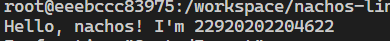
\includegraphics[width=0.6\textwidth]{images/hello.png}
	\caption{Hello Nachos}
	\label{fig:hello}
\end{figure}

\section{实现双向有序链表}

双向有序链表就是双向的、元素有序的链表。首先,按照上述加入hello的方法加入dllist
相关的文件。然后进行实现。为了保证链表有序,在插入时需要遍历链表、先找到元素应该插入的位置,
然后再插入。其余部分都按照相关文件中的注释进行实现即可。


\section{体验Nachos线程系统}

由于观察多线程访问中发生的问题需要多个线程、运行多次,而修改代码进行输出、在较多的日志中寻找
偶然发生的并发问题是一件相当需要时间的繁琐的事情。因此,需要对代码进行适当的修改和设计,在
保持代码可读性、可维护性的前提下插入辅助观察并发错误的业务逻辑,这一点需要较多的设计和改进。

因此,为了良好的完成实验、避免在繁琐的分析和查找中出错,更好地观察到各种并发问题,首先需要更好的
工具。因此,我将把我在这一节进行的工作按如下的顺序进行介绍:

\begin{enumerate}
	\item \texttt{\textbf{工具宏的定义}}:使用宏定义来简化在不同位置按需调用\texttt{Yield}的操作,以及输出调用\texttt{Yield}的位置等信息;
	\item \texttt{\textbf{使用上述工具宏改造双向有序链表}}:应用上述宏定义,方便简洁地实现能通过命令行参数指定代码中调用\texttt{Yield}的位置的功能;
	\item \texttt{\textbf{使用RAII自动检测并发错误}}:利用现代C++中常见的RAII范式完成自动的并发错误检查器,检查失序等比较难以直接观察和分析的并发错误;
	\item \texttt{\textbf{实验结果}}:错误内容的截图和讨论;
\end{enumerate}

\subsection{工具宏定义}

为了方便地观察并发中的现象,可以定义一些宏来使得代码更清晰。首先,为了观察不同位置调度后产生
的问题,需要调用\texttt{Yield},并且为了方便调试,还需要输出调用\texttt{Yield}的位置等信息,
以便于观察。因此可以定义一个宏,如代码~\ref{code:logyield}。
\begin{listing}[htb]
	\caption{logyield.h}
	\label{code:logyield}
	\begin{minted}{c}
#define DEBUG_YIELD_OUTPUT
#ifdef DEBUG_YIELD_OUTPUT
#define YIELD_AND_REPORT() \
do { \
printf("In function \"%s\":\n  Switch to another thread at code line %d!\n", __FUNCTION__, __LINE__); \
currentThread->Yield(); \
} while (0)
#else
#define YIELD_AND_REPORT() \
do { \
currentThread->Yield(); \
} while (0)
#endif
	\end{minted}
\end{listing}

在这段代码中,\texttt{DEBUG\_YIELD\_OUTPUT}作为开关,选择\texttt{YIELD\_AND\_REPORT}的内容。
如果定义了\texttt{DEBUG\_YIELD\_OUTPUT},则会输出调用\texttt{Yield}的位置等信息,否则不会输出。
为了获取这些位置信息,可以使用编译器预定义的宏\texttt{\_\_FUNCTION\_\_}和
\texttt{\_\_LINE\_\_}。
它们是调用位置函数的名称和代码行号。在这里,使用了do-while循环,是为了保证宏的语句块的完整性,不会在
替换时出错。

这样,在任何位置调用\texttt{YIELD\_AND\_REPORT},都会调用\texttt{Yield}并按需要输出调用位置的信息。

代码中许多部分都需要测试是否发生并发问题,因此,首先需要在\texttt{main.cc}中加入3个参数,分别是测试时
使用线程的数量t,测试的次数n,和需要\texttt{Yield}的位置标号,如代码~\ref{code:main}。
\begin{listing}[htb]
	\caption{main.cc}
	\label{code:main}
	\begin{minted}{c}
		case 't':		// number of threads
			threadnum = atoi(argv[1]);
			argCount++;
			break;
		case 'n':		// number of items
			itemnum = atoi(argv[1]);
			argCount++;
			break;
		case 'e': 	// type of error
			errorType = atoi(argv[1]);
			argCount++;
			break;
	\end{minted}
\end{listing}
这添加在\texttt{main.cc}95行开始for语句中的switch语句中。

在双向有序链表的实现中,需要判断存储需要\texttt{Yield}的位置标号,然后调用\texttt{YIELD\_AND\_REPORT}。
这一过程也可以用宏来简化,以减少代码中的重复。如代码~\ref{code:logyield2}。
\begin{listing}[htb]
	\caption{logyield.h}
	\label{code:logyield2}
	\begin{minted}{c}
	#define YIELD_ON_TYPE(t) \
	if (errorType == t)	 \
	{ \
		YIELD_AND_REPORT(); \
	} \
	\end{minted}
\end{listing}
这样,在需要判断并调用\texttt{YIELD\_AND\_REPORT}的地方,只需要调用\texttt{YIELD\_ON\_TYPE}即可。
传入的参数是标识当前位置的数值,它由命令行参数传入并放入变量\texttt{errorType}
中。

假设调用了\texttt{YIELD\_ON\_TYPE(1)},则会判断\texttt{errorType}是否为1,如果是,则调用。此时,
如果在执行nachos时传入了命令行参数\texttt{-e 1},则会在当前位置调用\texttt{YIELD\_AND\_REPORT}。

这样有了以上的宏定义,就可以用一行代码来标记当前位置、处理命令行参数,以及按需求调用\texttt{Yield}。

\subsection{使用上述工具宏改造双向有序链表}

接下来,为了方便观察并发中的现象,需要对双向有序链表进行改造。将上述工具宏实际应用到双向有序链表中。
并发的错误通常出现在读写链表节点的前后指针的位置。因此,为了观察这些位置的并发问题,需要在这些位置
插入上一节定义的\texttt{YIELD\_ON\_TYPE(标识ID)}。这里,标识ID的值可以自己定义,只要保证不同的位置
使用不同的标识ID即可。在启动Nachos时,将对应的标识ID作为参数传入,就可以在指定的位置调用\texttt{Yield}。

\subsection{使用RAII自动检测错误}

并发错误具有随机发生、频率不定的特点。为了引发并发错误,就需要运行多个线程、运行多次。在这个过程中,需要打出
大量的log来进行分析。这个过程较为繁琐,在大量的log中查找失序等问题并不容易。因此需要更好的方法检测问题。

其中一种方法是在在所有修改结点指针处插入各种检查代码。然而这种侵入式的修改方式需要对代码进行大量的修改,也会
影响程序结构使得代码难以理解。并且许多检查代码都是重复的,这会导致代码冗余。因此,需要一种非侵入式的自动检查
方案。

\subsubsection{什么是RAII}

RAII是C++中一种非常重要的编程技巧,它代表“资源获取即初始化”(Resource Acquisition Is Initialization)的缩写。其核心思想是利用对象的构造函数和析构函数,在对象生命周期结束时自动释放资源。通过RAII,程序员可以更加便捷、安全地管理内存、文件句柄、锁、网络连接等各种资源,从而避免因为手动管理资源而引入的错误。

RAII可以帮助避免许多常见的错误,如忘记释放资源、过早或过晚释放资源等。比如,如果程序员手动分配了内存但未在使用后及时释放,就会导致内存泄漏问题。而RAII可以在对象失效时自动调用析构函数,从而正确释放对象占用的资源,避免内存泄漏问题。

实现RAII需要将资源的管理封装在一个类中。例如,标准库对于动态内存的管理,实现了unique\_ptr等一系列智能指针
智能指针来确保在对象失效时自动释放内存。

RAII不仅可以避免资源泄漏问题,还可以提供异常安全保障。当程序抛出异常时,RAII可以确保已经分配的资源被正确释放,从而避免资源泄漏和内存泄漏等问题。这是因为在异常情况下,C++会自动调用对象的析构函数来释放资源,从而确保程序能够正确处理异常情况。

\subsubsection{使用RAII的方式自动检查并发错误}

虽然错误检查不是严格意义上的资源管理,但是它可以利用RAII的思想来实现。具体来说,可以将错误检查封装在一个类中,然后在类的构造函数中进行错误检查,而在析构函数中进行错误恢复。
这样,当进入相应的作用域中,就会自动进行错误检查,而在作用域结束时,就会自动再次检查,然后按需输出错误状态。
这样就可以避免手动检查和恢复错误。
这样,在调用端,只需要定义一个RAII对象,然后错误检查就能够自动执行,最大限度减少了错误检查实现的侵入性,使得错误检查更加简单、方便。对于链表失序、指针指向错乱等
问题,也能够更好地输出具体的错误信息,从而更加方便地进行分析。

在程序中,我实现了两种粒度的错误检测,分别是对链表的整体检查和对链表节点的检查。
链表的整体检查会检查头尾指针、是否有序等,节点级别的检查会检查节点的前后指针、
以及前后构成的三元组是否有序。

采用两种不同的粒度的检测,是因为链表结构的完整操作才能保证链表级别的不变性,例如整体的有序性。
然而,在链表操作之内的细分步骤中,局部的节点操作也有其不变性需要检查。例如前后局部的有序性、指针指向的一致性。
当然,在实践中,可以观察到链表级的错误检查没有发现任何问题,而节点级的错误检查则提供了一些有用的信息。

以节点级的错误检查为例,它的实现如代码~\ref{code:raiicheck}。在构造函数中,会检查节点的前后指针是否一致,
并且检查前后节点的三元组是否有序。在析构函数中,会再次检查节点的前后指针是否一致,并且检查前后节点的三元组是否有序。
例如要将其使用在链表的插入操作中,可以在插入操作的每个局部使用大括号\{和\}标记一个作用域,然后在其中定义一个RAII对象,
从而在作用域结束时自动进行错误检查。使用这种方法的实例如插入操作中的代码~\ref{code:insertexample}所示。使用这种方法检查,最好将作用域限定为能够维持节点
所需要维持的不变性的最小范围。这样,就更容易发现错误。
\begin{listing}[H]
	\caption{使用示例}
	\label{code:insertexample}
	\begin{minted}{c}
	{
		RAIINodeGuard _1(*last, "last");
		RAIINodeGuard _2(*element, "element");
		last->next = element;
		YIELD_ON_TYPE(19);
		element->prev = last;
		element->next = NULL;
		YIELD_ON_TYPE(20);
		last = element;
	}
	\end{minted}
\end{listing}

\begin{listing}[htb]
	\caption{节点级的错误检查}
	\label{code:raiicheck}
	\begin{minted}{c}

RAIINodeGuard::RAIINodeGuard(DLLElement& ele, char* name)
	: ele_(&ele), name_(name)
{
	printf("Thread %s enter guarded section for %s. ", currentThread->getName(), name_);
	if (ele_->prev || ele_->next)
	{
		if (!ele_->prev)
		{
			printf("It's first node.");
		}
		if (!ele_->next)
		{
			printf("It's last node.");
		}
	}

	printf("\n");
	test();
}

RAIINodeGuard::~RAIINodeGuard()
{
	test();
	printf("Thread %s exit guarded section for %s\n", currentThread->getName(), name_);
}

void RAIINodeGuard::test()
{
	if (ele_->prev && ele_->prev->next != ele_)
	{
		printf("%s has wrong previous relationship.\n", name_);
		ASSERT(false);
	}

	if (ele_->next && ele_->next->prev != ele_)
	{
		printf("%s has wrong next relationship.\n", name_);
		ASSERT(false);
	}

	int diff1 = ele_->prev ? ele_->key - ele_->prev->key : 0;
	int diff2 = ele_->next ? ele_->next->key - ele_->key : 0;
	if (diff1 && diff2 && diff1 * diff2 < 0)
	{
		printf("%s has wrong order. Values are: ", name_);
		if (ele_->prev)
		{
			printf("%d ", ele_->prev->key);
		}

		printf("%d ", ele_->key);

		if (ele_->next)
		{
			printf("%d ", ele_->next->key);
		}

		printf("\n");

		ASSERT(false);
	}
}
	\end{minted}
\end{listing}

\clearpage

\subsection{实验结果}

使用以上的措施,就可以方便地进行错误检查。在实验中,我尝试了不同的\texttt{Yield}位置之后,
发现了四类错误,它们分别是:
\begin{enumerate}
	\item 空指针造成的Segmentation Fauld
	\item 两次释放同一段内存导致的Double Free问题
	\item 链表指针的错乱
	\item 链表的失序
\end{enumerate}
输出错误信息如图~\ref{fig:errors}。其中,只有借助上述RAII错误检查才能发现后两种错误。
可见,将错误检查进行一定程度的自动化有利于更好地调试并发程序。

\begin{figure}[htb]
	\centering
	\caption{错误信息}
	\label{fig:errors}
	\begin{subfigure}[b]{0.4\textwidth}
		\centering
		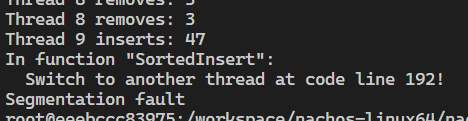
\includegraphics[width=0.9\textwidth]{images/segfault.png}
		\caption{空指针造成的Segmentation Fauld}
	\end{subfigure}
	\begin{subfigure}[b]{0.4\textwidth}
		\centering
		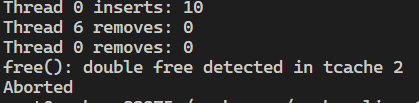
\includegraphics[width=0.9\textwidth]{images/dblfree.png}
		\caption{Double Free问题}
	\end{subfigure}
	\begin{subfigure}[b]{0.4\textwidth}
		\centering
		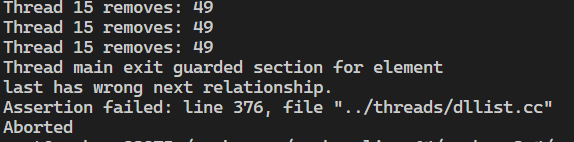
\includegraphics[width=0.9\textwidth]{images/wrongptr.png}
		\caption{链表指针的错乱}
	\end{subfigure}
	\begin{subfigure}[b]{0.4\textwidth}
		\centering
		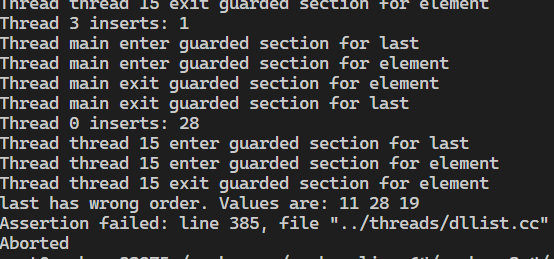
\includegraphics[width=0.9\textwidth]{images/wrongorder.png}
		\caption{链表的失序}
	\end{subfigure}
\end{figure}

\section{实验总结}

在本次实验中,我通过Docker实现了更方便的环境配置。实现双向有序链表,
并借助宏、RAII等功能更方便地观察了并发的问题。对并发可能产生的问题
有了进一步的理解。

\end{spacing}

\end{document}